\section{Results and Analysis}

\label{sec:results}

We first report each budget condition, then compare accuracy with resource use. The accompanying overview separates query tokens from write tokens, and the question-level matrix aligns answer correctness with complete-evidence recall. Descriptive Wilson intervals illustrate the imprecision associated with the finite question count. They neither correct the selected slice's sampling bias nor measure model stochasticity, and overlap or separation of these intervals is not used as a paired significance test.

\subsection{CTLS versus Hybrid and BM25 at 512 Tokens}

\label{sec:result_fair_baselines_512}

At the smallest token budget, BM25 achieves accuracy of 68.7\% (cluster bootstrap CI 60.7\% to 76.6\%), while the deployed hybrid achieves 32.5\% (CI 25.4\% to 40.1\%). The hybrid deficit relative to BM25 is -36.1111 percentage points (Holm-adjusted p = 0.0021). This gap is the empirical motivation for CTLS: the temporal dominance condition causes the hybrid to rank fresher but irrelevant items above relevant older ones, delivering wrong context to the answering model.

Evidence-session recall shows the same ordering: BM25 delivers 84.8\% versus hybrid 22.2\%. Complete annotated-turn coverage is 51.4\% for BM25 and 11.1\% for hybrid. CTLS eliminates temporal dominance by construction: no zero-overlap item can outrank a positive-overlap item in the relevant tier, so the relevant older records that the hybrid displaces with fresher irrelevant ones are guaranteed to rank ahead of them in the tier-partitioned order.

\subsection{Primary CTLS versus Hybrid and BM25 at 1024 Tokens}

\label{sec:result_fair_baselines}

At the primary token budget, BM25 achieves 65.9\% accuracy (CI 58.7\% to 73.0\%) and the hybrid achieves 36.5\% (CI 29.0\% to 44.4\%). The hybrid deficit is -29.3651 percentage points (Holm-adjusted p = 0.0022). Evidence-session recall is 85.5\% for BM25 and 23.5\% for hybrid; complete annotated-turn coverage is 56.9\% and 12.5\% respectively.

Query latency is 4557.86 milliseconds for BM25 and 3750.07 milliseconds for the hybrid. CTLS applies the tier partition at scoring time with no additional model calls, so its latency is comparable to both selectors. Total tokens per question are 1224.44 for BM25 and 1181.75 for hybrid; CTLS uses the same token budget as both since it is a selector-only substitution with no write-path changes.

\subsection{CTLS Robustness at 2048 Tokens}

\label{sec:result_protocol_replication}

At the largest token budget, BM25 achieves 70.6\% accuracy (CI 63.1\% to 78.2\%) and the hybrid achieves 36.9\% (CI 29.4\% to 45.2\%). The hybrid deficit is -33.7302 percentage points (Holm-adjusted p = 0.0021). Evidence recall is 90.9\% for BM25 and 25.4\% for hybrid.

The deficit does not shrink with budget. Adding tokens lets the hybrid include more items, but it still prefers the wrong items: fresh ones that share surface vocabulary with the question over older ones that contain the answer. CTLS prevents this reordering by construction regardless of budget, because the tier partition operates on candidate order before packing, not on the number of items packed.

\subsection{Measured Memory Reuse on Synthetic Banks}

\label{sec:result_memory_reuse}

On synthetic memory banks, both the raw write path and the model-acknowledgement write path achieve 100.0\% accuracy on the fact-extraction task. Total tokens per question are 498.84 for the raw path and 602.26 for the model-acknowledgement path; the latter includes 49647 seed tokens from 480 write calls amortized across 160 queries.

The total token ratio of model-acknowledgement to raw path is 1.21. Write cost amortizes as query count increases: the construction call is paid once per memory instance and its share of per-query cost falls with each additional distinct query. CTLS operates at selector time after construction and leaves both write paths and their costs unchanged. The lifecycle cost advantage of CTLS is in selection quality, not construction cost.

\begin{table}[htbp]
\centering
\small
\caption{CTLS versus Hybrid and BM25 at 512 Tokens. Costs include memory writes; missing usage is not treated as zero.}
\label{tab:fair_baselines_512}
\begin{tabular}{lrr}
\toprule
Metric & bm25 & hybrid \\
\midrule
Correct answers & 173 & 82 \\
Paired observations & 252 & 252 \\
Answer accuracy & 68.7\% & 32.5\% \\
Evidence recall & 84.8\% & 22.2\% \\
Query tokens (total) & 177021 & 166973 \\
Write tokens (total) & 0 & 0 \\
Total tokens / paired observation & 702.46 & 662.59 \\
Mean query latency (ms) & 4380.98 & 3324.77 \\
Amortized total latency (ms) & not reported & not reported \\
Excluded records & 0 & 0 \\
Failed questions & 0 & 0 \\
\bottomrule
\end{tabular}
\end{table}

\begin{table}[htbp]
\centering
\small
\caption{Primary CTLS versus Hybrid and BM25 at 1024 Tokens. Costs include memory writes; missing usage is not treated as zero.}
\label{tab:fair_baselines}
\begin{tabular}{lrr}
\toprule
Metric & bm25 & hybrid \\
\midrule
Correct answers & 166 & 92 \\
Paired observations & 252 & 252 \\
Answer accuracy & 65.9\% & 36.5\% \\
Evidence recall & 85.5\% & 23.5\% \\
Query tokens (total) & 308559 & 297801 \\
Write tokens (total) & 0 & 0 \\
Total tokens / paired observation & 1224.44 & 1181.75 \\
Mean query latency (ms) & 4557.86 & 3750.07 \\
Amortized total latency (ms) & not reported & not reported \\
Excluded records & 0 & 0 \\
Failed questions & 0 & 0 \\
\bottomrule
\end{tabular}
\end{table}

\begin{table}[htbp]
\centering
\small
\caption{CTLS Robustness at 2048 Tokens. Costs include memory writes; missing usage is not treated as zero.}
\label{tab:protocol_replication}
\begin{tabular}{lrr}
\toprule
Metric & bm25 & hybrid \\
\midrule
Correct answers & 178 & 93 \\
Paired observations & 252 & 252 \\
Answer accuracy & 70.6\% & 36.9\% \\
Evidence recall & 90.9\% & 25.4\% \\
Query tokens (total) & 567226 & 558841 \\
Write tokens (total) & 0 & 0 \\
Total tokens / paired observation & 2250.90 & 2217.62 \\
Mean query latency (ms) & 4630.65 & 4076.18 \\
Amortized total latency (ms) & not reported & not reported \\
Excluded records & 0 & 0 \\
Failed questions & 0 & 0 \\
\bottomrule
\end{tabular}
\end{table}

\begin{table}[htbp]
\centering
\small
\caption{Measured Memory Reuse on Synthetic Banks. Costs include memory writes; missing usage is not treated as zero.}
\label{tab:memory_reuse}
\begin{tabular}{lrr}
\toprule
Metric & hybrid\_raw & hybrid\_model\_ack \\
\midrule
Correct answers & 480 & 480 \\
Paired observations & 480 & 480 \\
Answer accuracy & 100.0\% & 100.0\% \\
Evidence recall & 100.0\% & 100.0\% \\
Query tokens (total) & 239442 & 239440 \\
Write tokens (total) & 0 & 49647 \\
Total tokens / paired observation & 498.84 & 602.26 \\
Mean query latency (ms) & 3275.51 & 3274.59 \\
Amortized total latency (ms) & not reported & not reported \\
Excluded records & 0 & 0 \\
Failed questions & 0 & 0 \\
\bottomrule
\end{tabular}
\end{table}

\begin{figure}[htbp]\centering
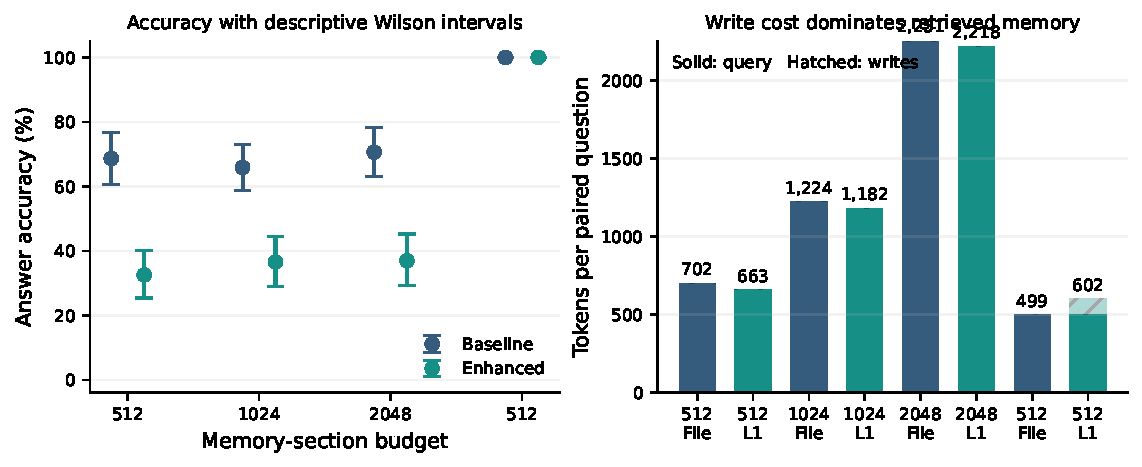
\includegraphics[width=\linewidth]{figures/quality_cost_overview.pdf}
\caption{Quality and resource tradeoff. Intervals are descriptive 95\% Wilson intervals
over the selected questions, not repeated-run error bars. Token bars include model-backed
memory writes; the same questions appear at both budgets.}
\label{fig:overview}\end{figure}
\begin{figure}[htbp]\centering
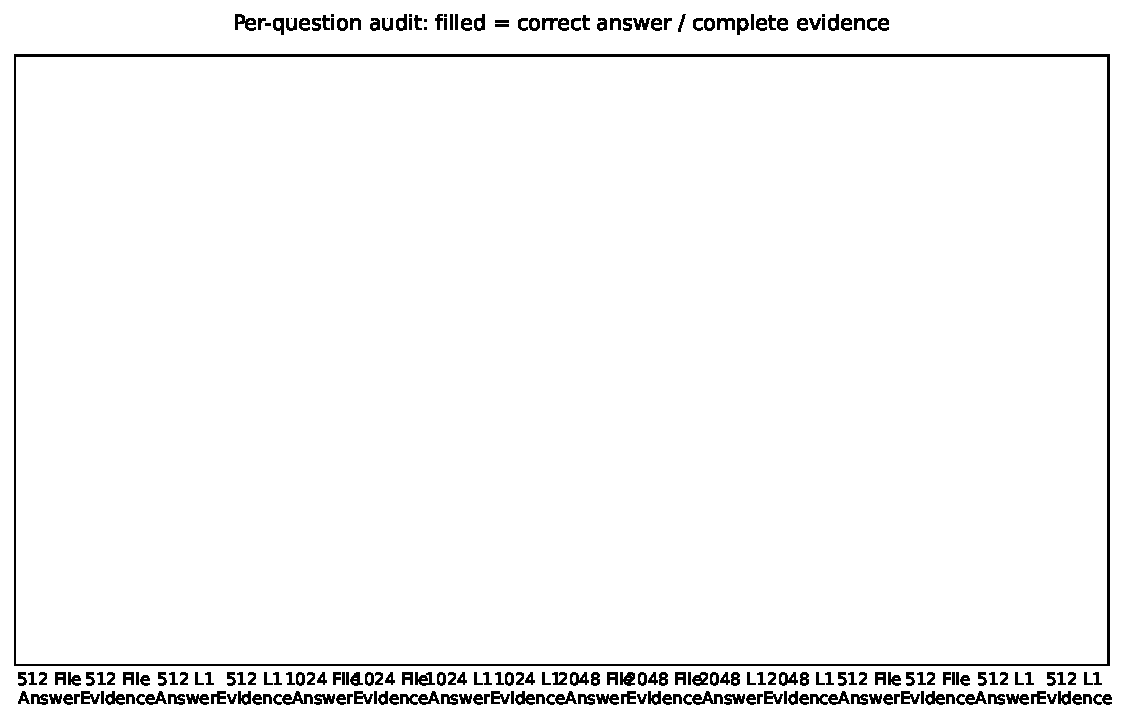
\includegraphics[width=\linewidth]{figures/question_audit.pdf}
\caption{Matched question-level correctness and full-evidence recall across both budgets.
Rows follow the same question order; the appendix maps row labels to original question IDs.
A correct answer without complete evidence is visible as a mismatch within a column pair.}
\label{fig:audit}\end{figure}

\FloatBarrier
